%
% BUS 338: Foundations of Innovation - A Course Overview
% Section: Product
%
% Author: Jeffrey Leung
%

\section{Product}
	\label{sec:product}
\begin{easylist}

& \textbf{Whole product:} Basic product in addition to other factors which create a reason to buy or augment the basic product
	&& E.g. Installation, configuration, integration, maintenance, customer support, other compatible products
	&& Composed of several layered perceptions (see figure~\ref{fig:whole-product})
		&&& \textbf{Generic product:} Basic product provided to customer with no additional features
			&&&& E.g. Wardrobe as individual pieces
		&&& \textbf{Expected product:} Basic product with features which the customer assumes they will receive
			&&&& E.g. Wardrobe pre-built or with a worker to assemble it
		&&& \textbf{Augmented product:} Product with all features included to maximize the value provided to the customer
			&&&& E.g. Wardrobe delivered to the house and assembled by the worker, with a warranty
		&&& \textbf{Potential product:} Possibilities of additional features beyond the scope or abilities of the original product
			&&&& E.g. Wardrobe with built-in light and clothes categorization system
	&& Early adopters do not require a full product, but pragmatists often do

\begin{figure}[!htb]
	\centering
	\caption{Whole Product}
	\label{fig:whole-product}
	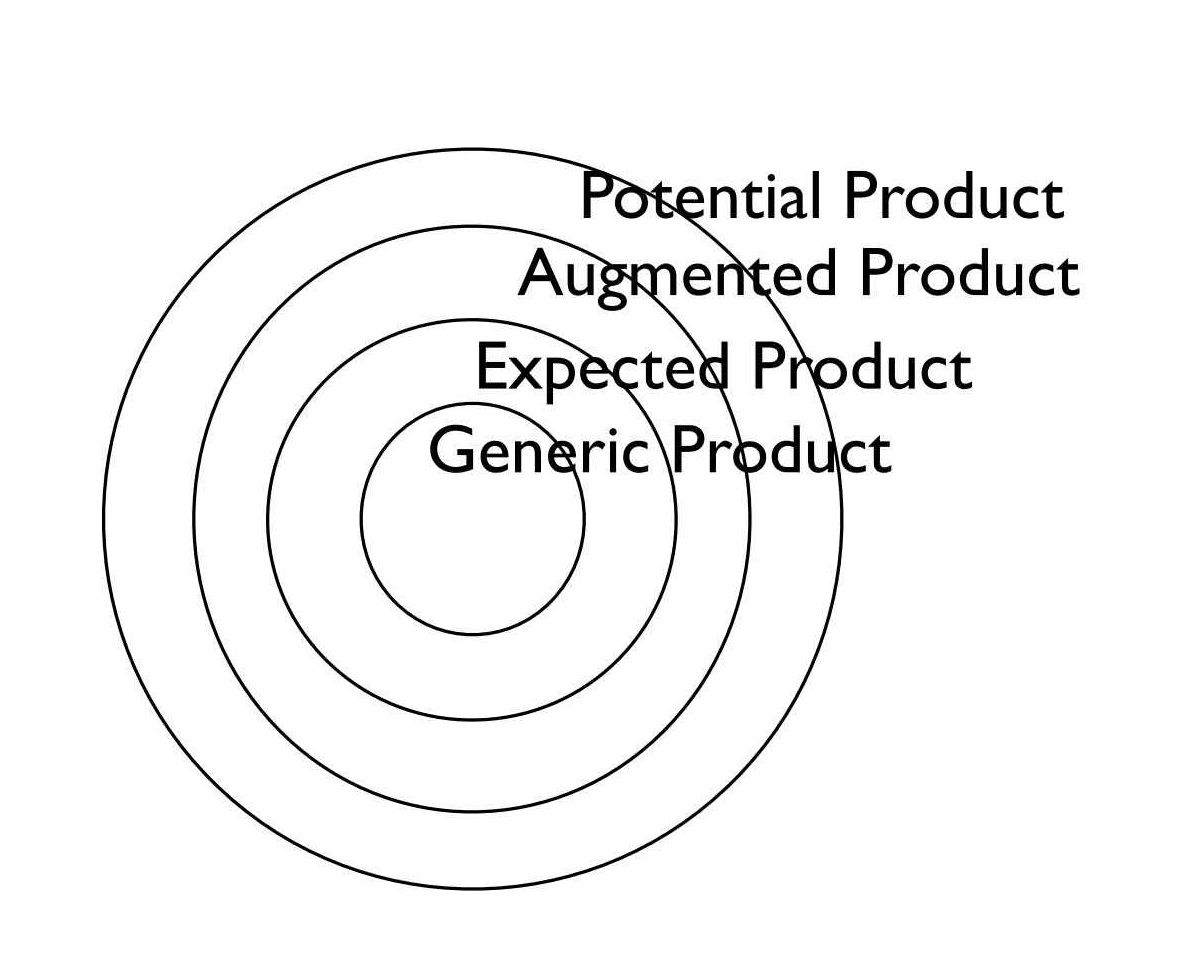
\includegraphics[width=0.7\textwidth]{whole-product}
\end{figure}

& Product characteristics:
	&& Features: Description, specifications, informative data (e.g. speed, dimensions, colors, models)
	&& Product benefits and key customer value: Reasons for using the solution and their importance (e.g. save time or money)
	&& Enhance the way that features add value to customers

& Match the prioritized customer needs to the product's benefits
	&& Needs must be important to the customer
	&& The match between benefits and needs should excel among the competition

\end{easylist}
\clearpage
